\section{Simulation Study: Internal Validation and Benchmarking}
\label{sec:results}

\subsection{Simulation Setup and Ground-Truth Parameters}

We generated a \textit{synthetic ICU dataset} for patients observed over 168 hours. For PKPD estimation experiments, we used $N=1000$ patients treated with the stochastic, stepwise dose-switching treatment pattern. For all other experiments, we simulated $N=2000$ subjects treated with either closed-loop control or no treatment, with probabilities of being assigned to each group either uniformly random when simulating a true RCT, or assigned as described in Section~\ref{sec:TreatmentAssignment} when simulating observational data.


\subsection{Simulated Cohorts and the Confounding Problem}
\label{sec:cohorts}

All results in this section are obtained from synthetic cohorts generated by the model of
Section~\ref{sec:datagen}, in which the true causal effect of each policy is known by construction.
We generated two parallel cohorts of $N = 2000$ patients each over a 168-hour horizon, differing only
in how treatment was assigned. In the \textbf{simulated trial} cohort, patients were assigned to
closed-loop control at $\theta = 0.1$ or to no treatment with equal probability, independently of
patient characteristics. In the \textbf{simulated observational} cohort, assignment followed the
confounded mechanism of Section~\ref{sec:TreatmentAssignment}, in which sicker patients are
preferentially treated, and informative censoring was applied. A separate cohort of $N = 1000$
patients receiving stochastic stepwise dose-switching was generated for the PK/PD estimation
experiments of Section~\ref{sec:pkpd-results}.

Because assignment in the trial cohort is randomized and that cohort is uncensored, the difference in
168-hour survival between its arms requires no modeling: it is obtained directly as the difference in
the proportion surviving. This quantity is the ground truth of the simulation, and it is the benchmark
against which every observational estimator below is measured.

\paragraph{Monte Carlo replication of the confounding effect.}
Because a single simulated cohort gives only one draw from the data-generating process, we replicated
the entire generation-and-analysis procedure over 400 independent replications (200 seeds in each of
the MATLAB and Python implementations, $N = 2000$ per cohort). Table~\ref{tab:multiseed} reports the
resulting sampling distributions. The ground-truth policy contrast averaged $+14.6$ percentage points
(Monte Carlo SE $0.11$), and naive Kaplan--Meier analysis of the confounded cohort averaged $+1.0$
points (MCSE $0.16$): confounding by indication eliminated 93\% of the true treatment effect. In
39\% of replications the attenuation was severe enough to reverse the sign of the estimate, so that
naive analysis indicated net harm from a treatment that was in fact beneficial. The two independent
implementations agreed on all three quantities to within Monte Carlo error (Welch $p \geq 0.06$;
two-sample Kolmogorov--Smirnov $p \geq 0.11$).

We report these as distributions rather than as a single cohort's values deliberately. Sign reversal
is a property of a substantial minority of replications, not of the data-generating process as such,
and the stable and more informative characterization of the confounding in this simulation is the
93\% attenuation of the true effect. All figures in this section display one representative cohort;
the quantities that carry the paper's claims are the replicated estimates in
Table~\ref{tab:multiseed}.

\begin{table}[htbp]
\centering
\begin{tabular}{lrrrr}
\toprule
Quantity & Mean & SD & MCSE & 95\% range \\
\midrule
Ground-truth ATE (randomized cohort)   & $+14.57$ & $2.17$ & $0.109$ & $[+10.81, +18.70]$ \\
Naive Kaplan--Meier ATE (observational) & $+1.00$  & $3.12$ & $0.156$ & $[-5.33, +6.90]$ \\
Bias of the naive estimator             & $-13.57$ & $3.79$ & $0.189$ & $[-21.24, -6.52]$ \\
\bottomrule
\end{tabular}
\caption{Sampling distribution of the ground-truth and naive treatment effects over 400 independent
simulated replications (200 seeds each in the MATLAB and Python implementations; $N=2000$ per cohort;
168-hour endpoint). All values are percentage points. The naive estimator retains 7\% of the true
effect on average and reverses its sign in 156/400 (39\%) of replications. All data are simulated.}
\label{tab:multiseed}
\end{table}

Figure~\ref{fig:swimmer_survival_rct} illustrates one representative pair of cohorts. In the trial cohort, the similar early coloring of the two arms in the
disease-burden heatmap reflects successful randomization: treated and untreated patients begin with
comparable severity. The untreated natural history is monophasic, rising rapidly and then tapering,
and although the disease eventually resolves without treatment, many patients die first. Treatment
intensity is highest where disease intensity is highest, reflecting the closed-loop policy, and the
clean separation between arms reflects perfect adherence and no dropout. In the observational cohort,
the treated group is visibly more severe from the outset, because clinicians in that cohort
preferentially treat sicker patients. The consequence is the central difficulty this paper addresses:
patients most likely to benefit from treatment are also most likely to die regardless of it, so
treatment appears harmful or ineffective under naive analysis.

\begin{figure}[htbp]
   \centering
   \noindent\textbf{(A) Simulated randomized trial}\par\vspace{0.2em}
   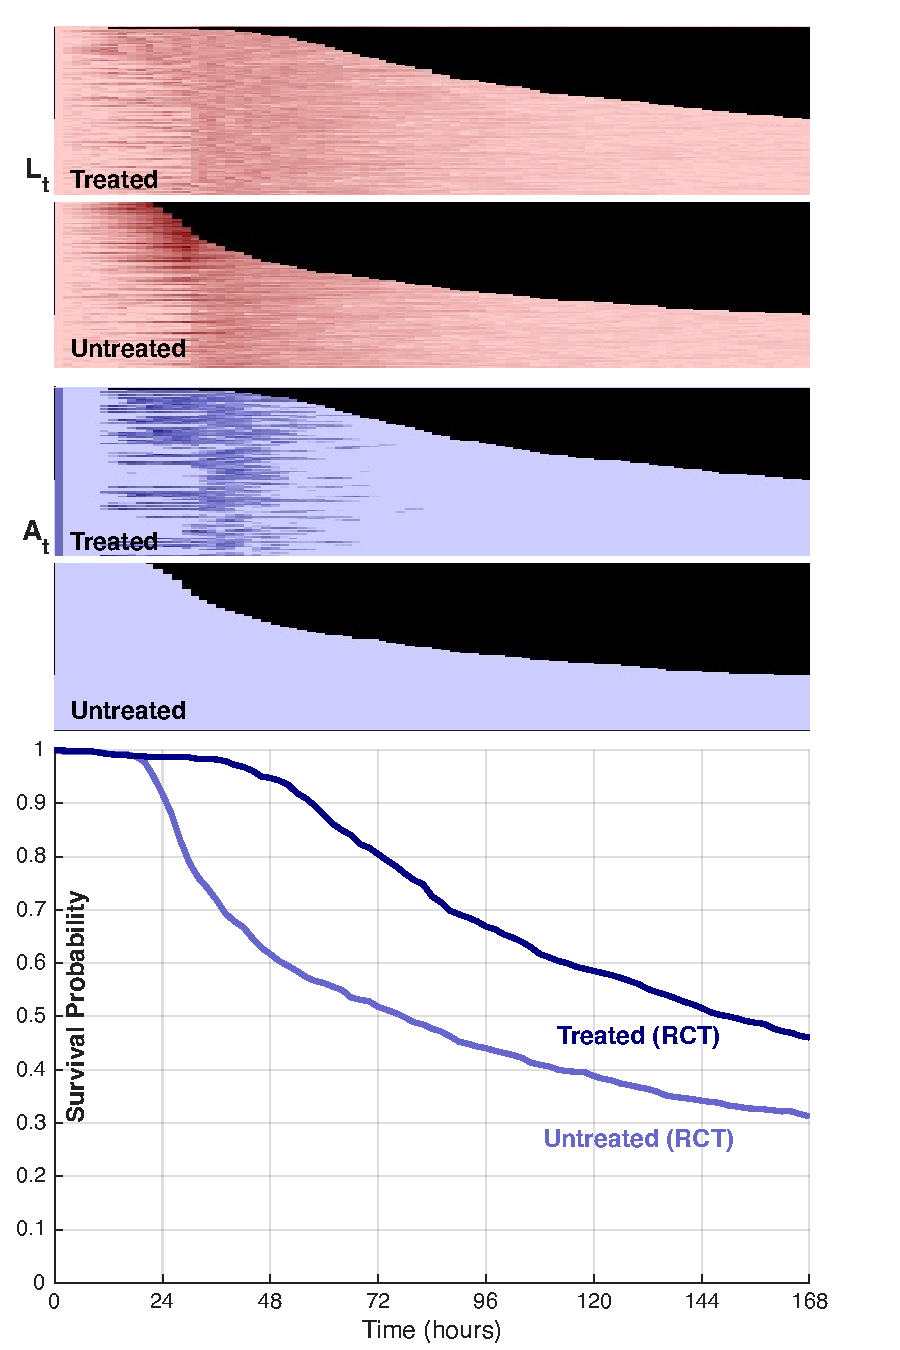
\includegraphics[width=0.68\textwidth,height=0.38\textheight,keepaspectratio, trim = 5pt 0pt 5pt 5pt, clip]{Fig3_swimmer_survival_plot_RCT.pdf}

   \vspace{0.9em}

   \noindent\textbf{(B) Simulated observational cohort}\par\vspace{0.2em}
   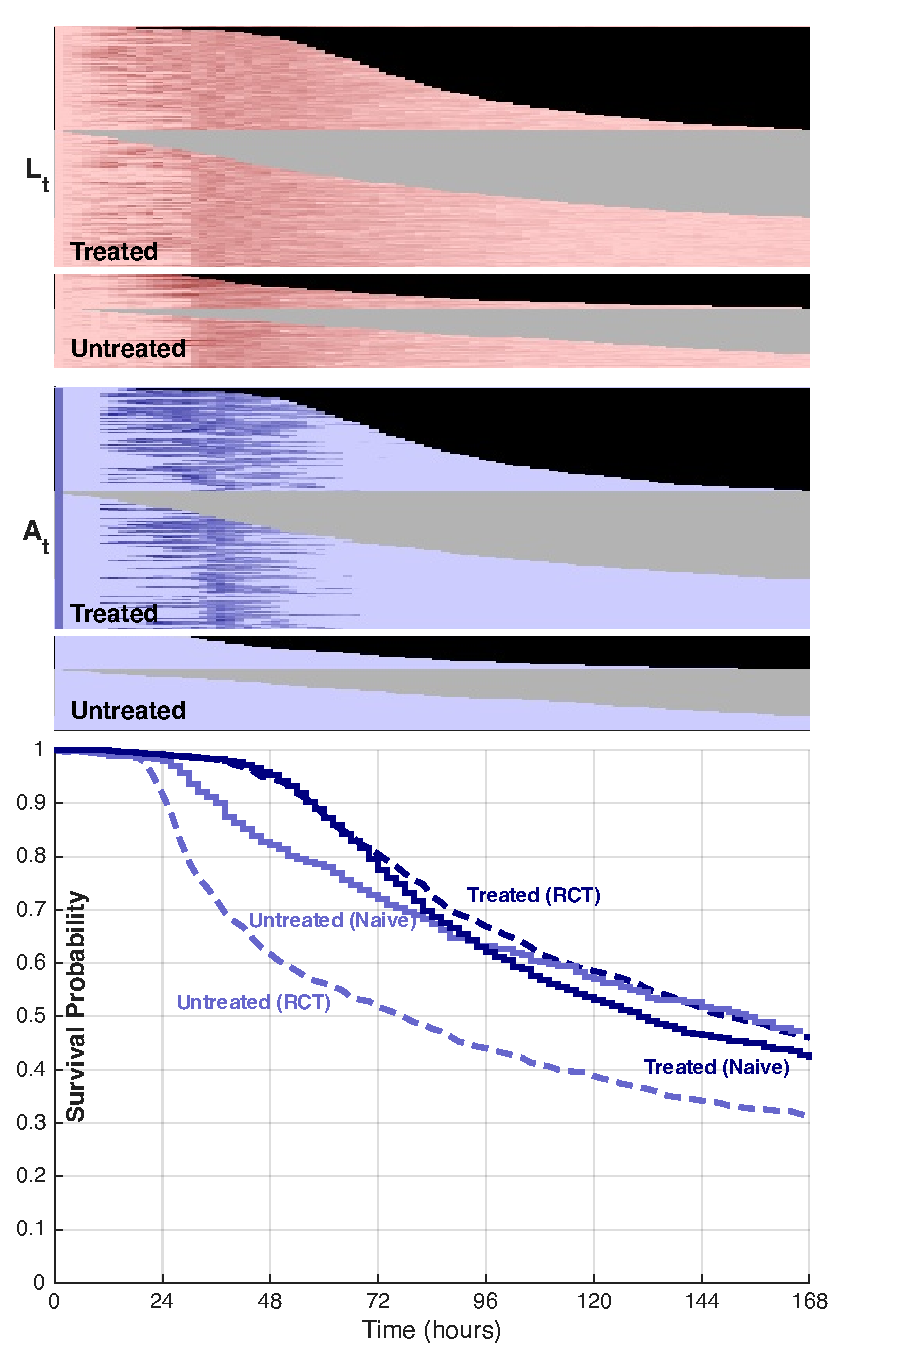
\includegraphics[width=0.68\textwidth,height=0.38\textheight,keepaspectratio, trim = 5pt 0pt 5pt 5pt, clip]{Fig4_swimmer_survival_plot_Obs_Naive.pdf}

   \caption{\textbf{Simulated trial and observational cohorts (one representative replication).}
Each row of a heatmap is one patient over 168 hours; within each block, patients are sorted by
survival time, producing the characteristic waterfall pattern. In every heatmap the treated arm is
shown in the upper block and the untreated arm in the lower block. \textbf{(A) Simulated randomized
trial} ($N = 2000$). Upper pair: epileptiform-activity burden $L_t$, light red indicating low burden
and dark red high; black indicates death. Middle pair: treatment intensity $A_t$, light blue
indicating none and dark blue high. Bottom: Kaplan--Meier survival by arm. Because assignment is
randomized and the cohort uncensored, the 168-hour survival difference is the ground-truth causal
effect of the simulation's data-generating process. \textbf{(B) Simulated observational cohort}
($N = 2000$), generated from the same disease and PK/PD models but with confounded treatment
assignment and informative censoring (gray). Baseline severity is higher among treated patients,
reflecting preferential treatment of sicker patients. Bottom: solid lines show the naive
Kaplan--Meier estimate; dashed lines reproduce the ground truth from panel~A. Values for this single
replication fall within the sampling distributions of Table~\ref{tab:multiseed}, which are what the
paper's claims rest on. All data are simulated.}
   \label{fig:swimmer_survival_rct}
\end{figure}

We emphasize that both cohorts are simulated, and that the confounding mechanism producing the
attenuation is one we specified; its magnitude is therefore a design choice rather than an empirical
finding about ICU practice. Its purpose is to provide a setting severe enough to discriminate between
estimators.

\subsection{Internal Validation: PK/PD Parameter Recovery}
\label{sec:pkpd-results}

We first evaluate the accuracy and robustness of our PKPD parameter estimation framework before assessing its performance in causal inference applications. This two-step evaluation ensures that any biases in downstream causal effect estimates can be attributed to the causal inference method rather than parameter estimation errors.

\subsubsection{Parameter Recovery Accuracy}

Figure~\ref{fig:L_prediction}A compares mean absolute percentage errors for each of the six population parameters and $k_e$ across estimation strategies. The fixed-$k_e$ oracle method (green) achieves the lowest overall MAPE (0.2\%), with zero error for $k_e$ by design, and the highest $L_0$ correlation (0.583). The two-stage corrected method (dark blue) performs nearly as well (MAPE 0.9\%, $k_e$ error 3.5\%), substantially outperforming the raw two-stage variant (MAPE 4.2\%, $k_e$ error 26.6\%) and the joint estimation approach (MAPE 22.9\%).

The superior performance of the corrected two-stage approach reflects the benefits of sequential estimation: first, establishing the natural history of the disease from untreated patients, then leveraging dose-switching variation to identify PKPD parameters. Joint estimation struggles with parameter interactions and local optima, while the raw two-stage method suffers from systematic bias in $k_e$ estimation that propagates to other parameters. The bias correction factor of 1.41, determined by regressing true $k_e$ values in the raw two-stage estimates, effectively compensates for systematic underestimation in the raw $k_e$ estimates, delivering the best practical performance for real-world applications where the true elimination constant is unknown.

\begin{figure}[htbp]
\centering
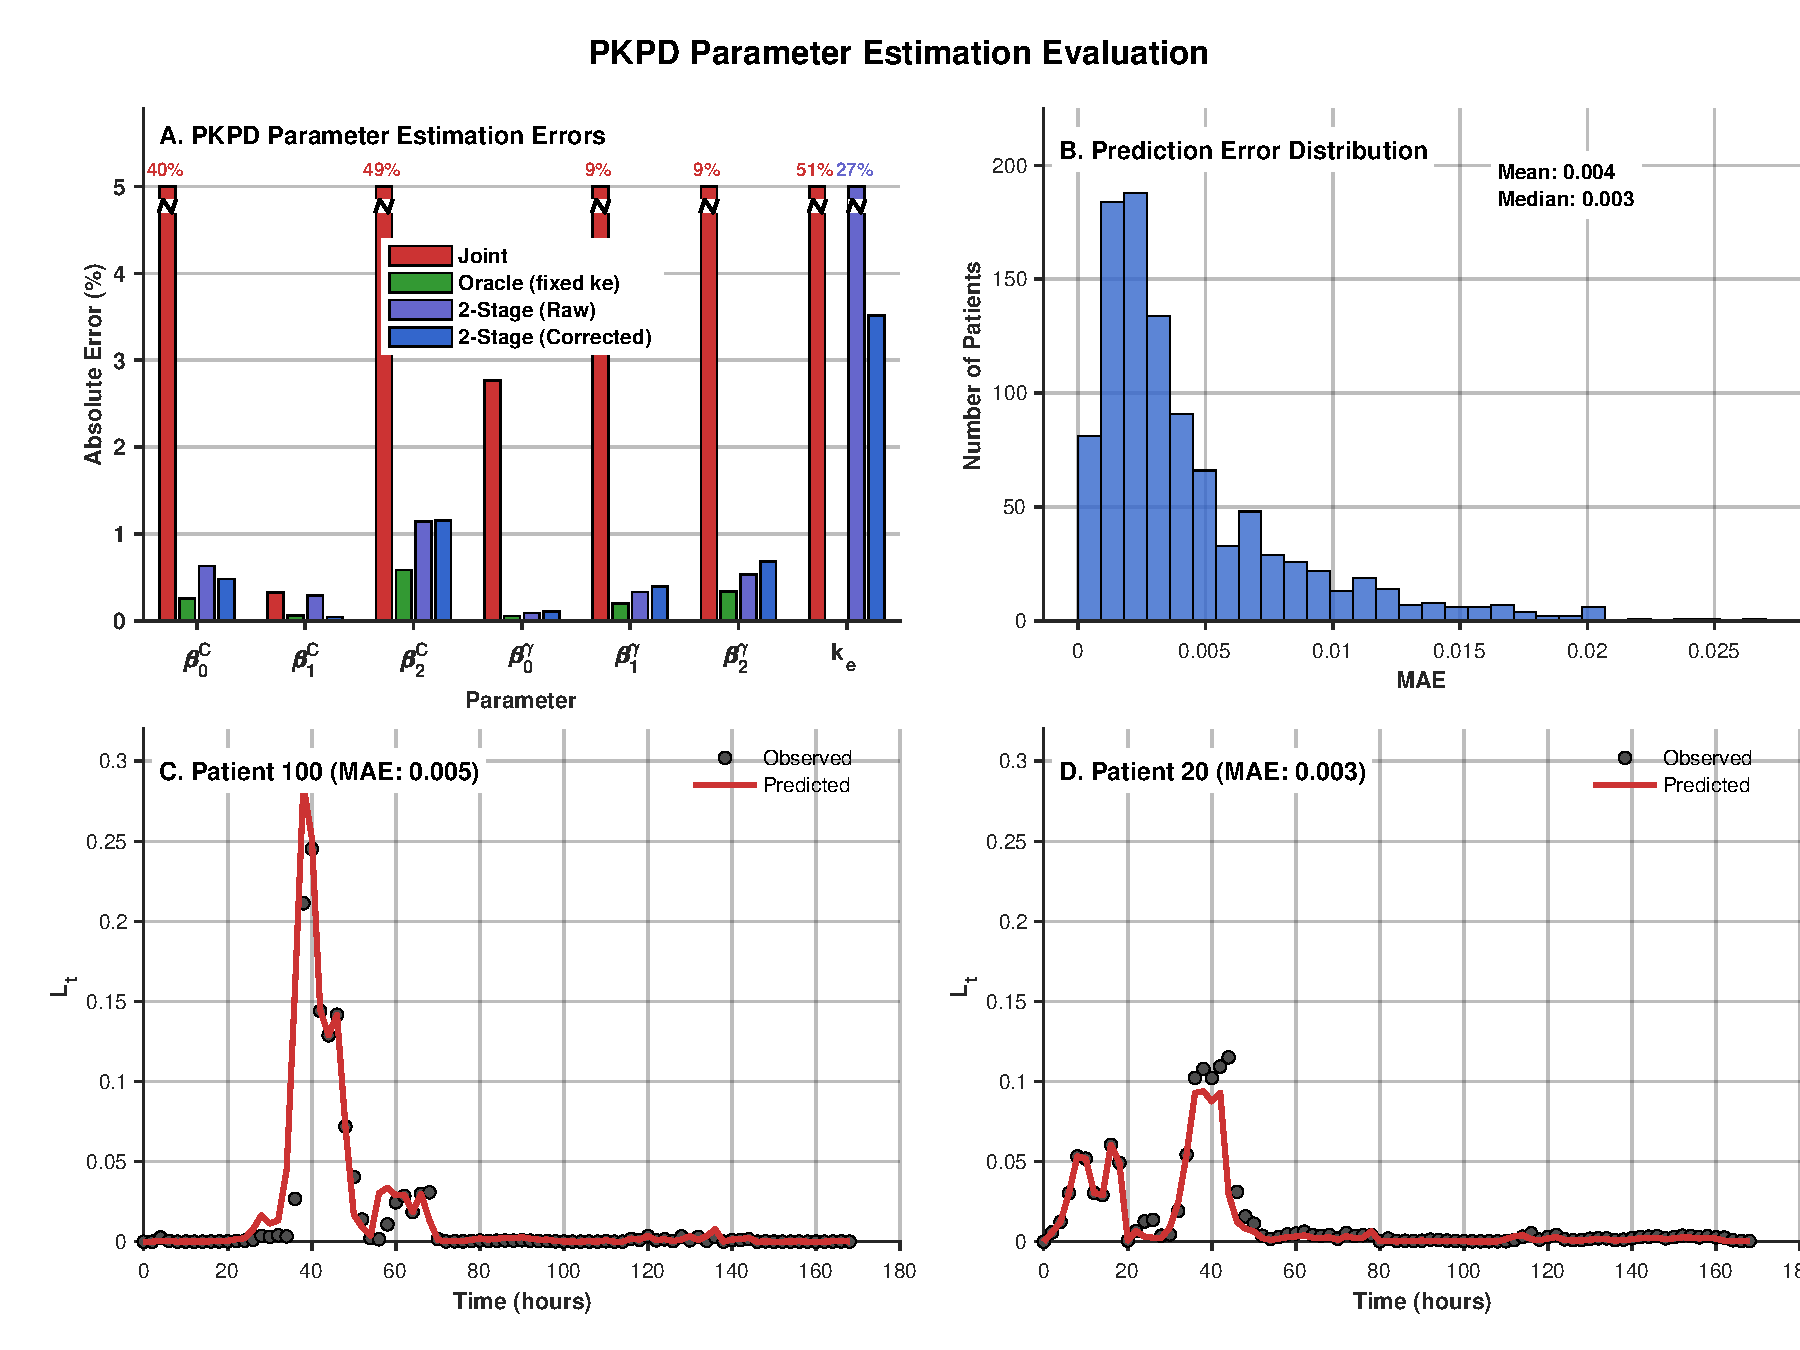
\includegraphics[width=\textwidth]{Fig_Combined_PKPD_Analysis.pdf}
\caption{(A) Absolute percentage errors in PKPD parameter estimates. Grouped bars show results for all six population parameters and $k_e$. The y-axis is truncated at 5\%; taller bars display their true values above. The oracle method (green) has zero $k_e$ error by definition. (B) Distribution of prediction accuracy values measured as mean absolute error (MAE) for $L_t$ using the PKPD parameters estimated using the 2-stage corrected method. (C,D) Two example predicted patient trajectories (red) compared with the observed values (black circles).}
\label{fig:L_prediction}
\end{figure}

\subsubsection{Predictive Performance and Model Validation}

Using the estimated PKPD parameters, we evaluated predictive accuracy for $L_t$. The corrected two-stage estimates yield visually close fits with good overall performance ($R^2 = 0.899$, Figure~\ref{fig:L_prediction}D). The prediction accuracy shows mean MAE of 0.004 (median 0.003) with mean MAPE of 52.6\% (median 45.3\%, interquartile range 37.0--56.1\%). While the MAPE values appear high, this reflects the challenge of predicting a highly suppressed signal where small absolute errors become large relative errors when $L_t$ values are near zero due to effective treatment. The strong $R^2$ value and low absolute MAE confirm that the model captures the essential dynamics despite this relative error inflation.

The mixed-effects coefficients defining how patient-specific PKPD parameters depend on covariates are recovered accurately (MAPE 0.9\%). This means we accurately recover the systematic relationships between patient characteristics (age, SOFA score) and their pharmacodynamic sensitivity. The moderate correlations between true and estimated individual patient parameters ($C_{50}$ correlation 0.532, Hill coefficient $\gamma$ correlation 0.328) reflect the inherent difficulty of recovering patient-specific random effects from limited dose-switching data, rather than errors in the underlying covariate-parameter relationships.

\subsubsection{Uncertainty Quantification}

We assessed parameter uncertainty using patient-level nonparametric bootstrap resampling ($B=1000$ replicates). Bootstrap resampling was performed at the patient level to preserve the within-patient correlation structure while allowing for realistic assessment of sampling variability. For each bootstrap replicate, we re-estimated all PKPD parameters using the corrected two-stage method.

The resulting 95\% interval for the elimination constant $k_e$ was $[0.47, 0.53]$ against a true value of $0.5$, and the intervals for the mixed-effects coefficients ($\beta^C_0$, $\beta^C_1$, $\beta^C_2$, $\beta^g_0$, $\beta^g_1$, $\beta^g_2$) were correspondingly narrow, reflecting the identification afforded by the dose-switching design.


\subsection{Internal Validation: Causal Effect Recovery}
\label{sec:gformula-results}
Having established accurate estimation of disease dynamics and PKPD parameters, we now assess whether the g-formula recovers the ground-truth causal effect of the simulation from the confounded observational cohort of Section~\ref{sec:cohorts}.

\subsubsection{Recovery of the Simulation Ground Truth}
The g-formula recovers the ground-truth effect closely despite confounding severe enough to eliminate the effect under naive analysis. For our primary comparison of aggressive treatment ($\theta = 0.1$) versus no treatment, the g-formula estimates show treated group survival of 46.3\% at 168 hours compared to 32.1\% in the untreated group, yielding an average treatment effect (ATE) of +14.2\%. 

This closely approximates the ground truth from the randomized controlled trial (treated survival 46.0\% vs. untreated 31.2\%, ATE +14.8\%), representing a recovery error of only 0.6 percentage points or 3.8\% relative error. Figure~\ref{fig:gformula_recovery} shows the estimated and ground-truth survival curves over the full follow-up. This recovery establishes that the estimator is consistent for the target parameter under the conditions of this simulation---correctly specified component models, measured confounding, and the censoring mechanism used to generate the data. It does not establish that these conditions hold in ICU data; Section~\ref{sec:misspec} discusses which of them are most likely to fail.

To assess the uncertainty quantification we repeated the entire generate--estimate--emulate procedure
across 100 independently simulated cohorts, re-estimating the mortality and natural-history models in
each. Across these replications the g-formula estimate had a standard deviation of 2.32 percentage
points, against a bootstrap standard error of 2.16 points obtained from a single cohort (ratio 0.93).
A nominal 95\% interval constructed from the bootstrap standard error contained the population
estimand in 92\% of replications (95\% CI 87--97\%), so the intervals are approximately calibrated at
the nominal level. We note that this is a lower bound on total sampling variability: as in the
bootstrap itself, the pharmacokinetic--pharmacodynamic fit is held at its point estimate rather than
re-estimated, so uncertainty in that component is not propagated into the interval.

Across the same 100 replications the estimator's mean was $+15.02$ percentage points against a mean
ground truth of $+14.30$, a bias of $+0.72$ points (95\% CI $+0.10$ to $+1.34$), or about 5\% of the
effect being estimated. The bias is small relative to the effect but statistically distinguishable
from zero, and it is upward: in this data-generating process the g-formula slightly overstates the
benefit of suppression.

One point of interpretation matters here. The g-formula estimate is obtained by forward simulation
from fitted models and therefore targets the population-level estimand rather than the realized
treatment effect of the particular cohort it was fitted on. Because a single cohort's realized effect
is itself a draw with non-trivial variability (SD 2.25 points across the replications reported here),
scoring the estimator against one cohort's realized value conflates estimator bias with that cohort's
sampling noise.

The magnitude of the correction is best read against the replicated naive estimates of Table~\ref{tab:multiseed} rather than against a single cohort. Naive Kaplan--Meier analysis retained on average only 7\% of the true effect ($+1.0$ against $+14.6$ percentage points), and in this representative cohort it indicated net harm ($-4.8\%$). The g-formula recovers the ground truth in the same data, a correction of roughly 13.6 percentage points on average and 19.6 points in the cohort shown.

\begin{figure}[H]
\centering
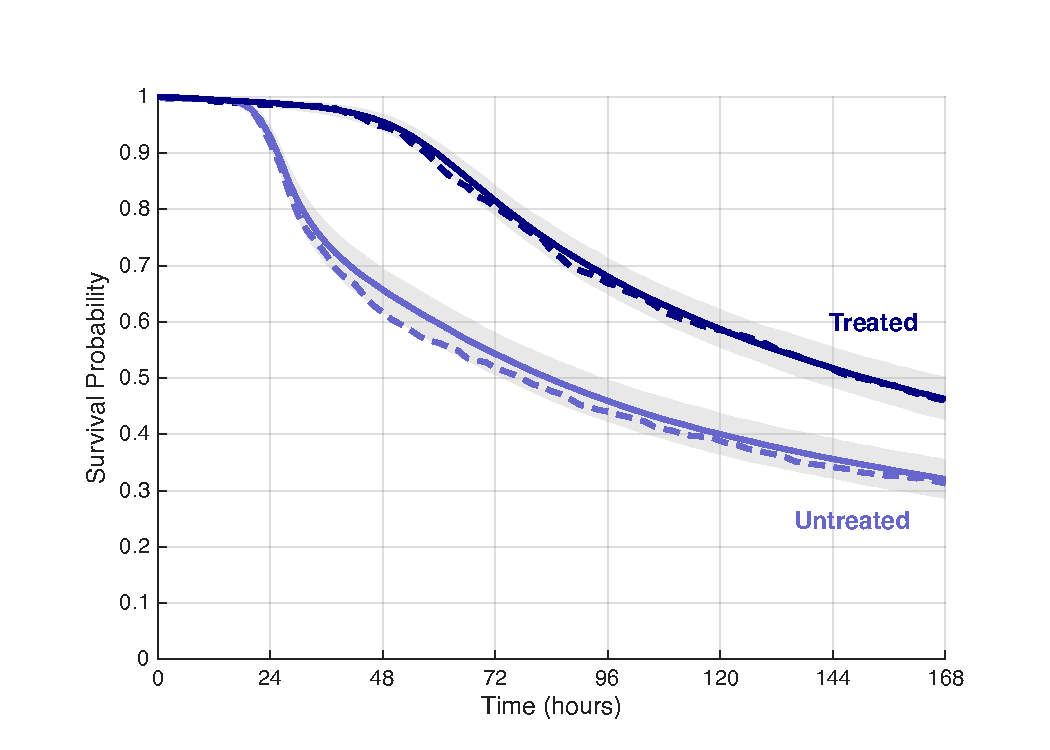
\includegraphics[width=\textwidth, trim=20pt 0pt 20pt 25pt, clip]{Fig_gformula_corrected_survival_curves.pdf}
\caption{\textbf{G-formula recovery of the simulation ground truth.} Survival probability curves over 168 hours comparing g-formula estimates from observational data (solid lines with 95\% CI) vs. ground truth from simulated RCT (dashed lines). In this representative cohort the g-formula achieves ATE $=+14.2\%$ against a ground truth of $+14.8\%$ (relative error 3.8\%). All data are simulated.}
\label{fig:gformula_recovery}
\end{figure}

\subsection{Policy-Space Exploration}
\label{sec:policy-space}

We next demonstrate the application of our framework: identifying optimal treatment strategies and revealing treatment effect heterogeneity across patient subgroups. This illustrates a second use of the framework: rather than evaluating one pre-specified contrast, it can be swept across a family of policies. In real data this would generate candidate strategies for prospective testing; here it demonstrates only that the sweep is computationally well posed and recovers the optimum of the process we specified.

\subsubsection{Optimization of Treatment Intensity}

While aggressive treatment ($\theta = 0.1$) demonstrates clear benefit over no treatment, this raises a natural question: is this particular target optimal, or could patients benefit from more or less aggressive suppression? Figure~\ref{fig:policy_space}A addresses this optimization question, revealing that our initial aggressive treatment ($\theta = 0.1$) is suboptimal.

The optimum of the simulated process occurs at $\theta = 0.02$---more aggressive suppression that yields an ATE of approximately +20.3\% at 168 hours, substantially improving upon the +14.8\% achieved with $\theta = 0.1$. Critically, the relationship between treatment intensity and survival is non-monotonic: while moderate to aggressive suppression improves outcomes, attempting to completely eliminate disease activity ($\theta = 0$) results in net toxicity with an ATE of $-8.9\%$, performing worse than no treatment.

This inverted-U relationship highlights the fundamental trade-off between disease control and treatment toxicity that characterizes many critical care interventions. The optimal treatment threshold represents the point where the marginal benefit of additional disease suppression equals the marginal harm from increased drug exposure.


\subsubsection{Patient-Specific Treatment Effects and Heterogeneity}
Figure~\ref{fig:policy_space}B compares counterfactual survival under a \emph{family of closed-loop treatment policies}, rather than across patient risk strata. In all cases, treatment follows the same closed-loop control policy, and curves differ only in the target epileptiform activity threshold $\theta$, which parameterizes the policy being evaluated.

While the simulated optimum of $\theta = 0.02$ is the best strategy for the average simulated patient, critical care populations exhibit substantial heterogeneity in disease and treatment susceptibility. Figure~\ref{fig:policy_space}B systematically explores how optimal treatment strategies vary across patient types, indexed by their susceptibility to cumulative disease harm (horizontal axis) and cumulative drug harm (vertical axis).

Across the simulated grid of disease-harm and drug-harm susceptibilities, the policy contrast ranges from $-8.9\%$ to $+71.6\%$. The boundary separating regions where suppression helps from regions where it harms is a direct consequence of the two-parameter harm model specified in Section~\ref{sec:outcome-model}; its position carries no information about where such a boundary would lie in patients. What the figure demonstrates is that the framework \emph{localizes} such a boundary when one exists, which is the property that would be useful in real data.

Applying the threshold that is optimal for each simulated patient, rather than a single population-wide threshold, yields a policy contrast of $+31.7\%$ versus $+20.3\%$. That an individualized policy outperforms a uniform one inside a simulation with heterogeneous, known patient parameters is expected by construction rather than surprising: the individualized policy has access to the generating parameters. The quantity of interest is not the margin itself but whether the framework recovers the individualized optimum when those parameters must be estimated, which is what Section~\ref{sec:pkpd-results} assesses.

\begin{figure}[p]
\centering
\noindent\textbf{(A) Sweep over the target threshold $\theta$}\par\vspace{0.2em}
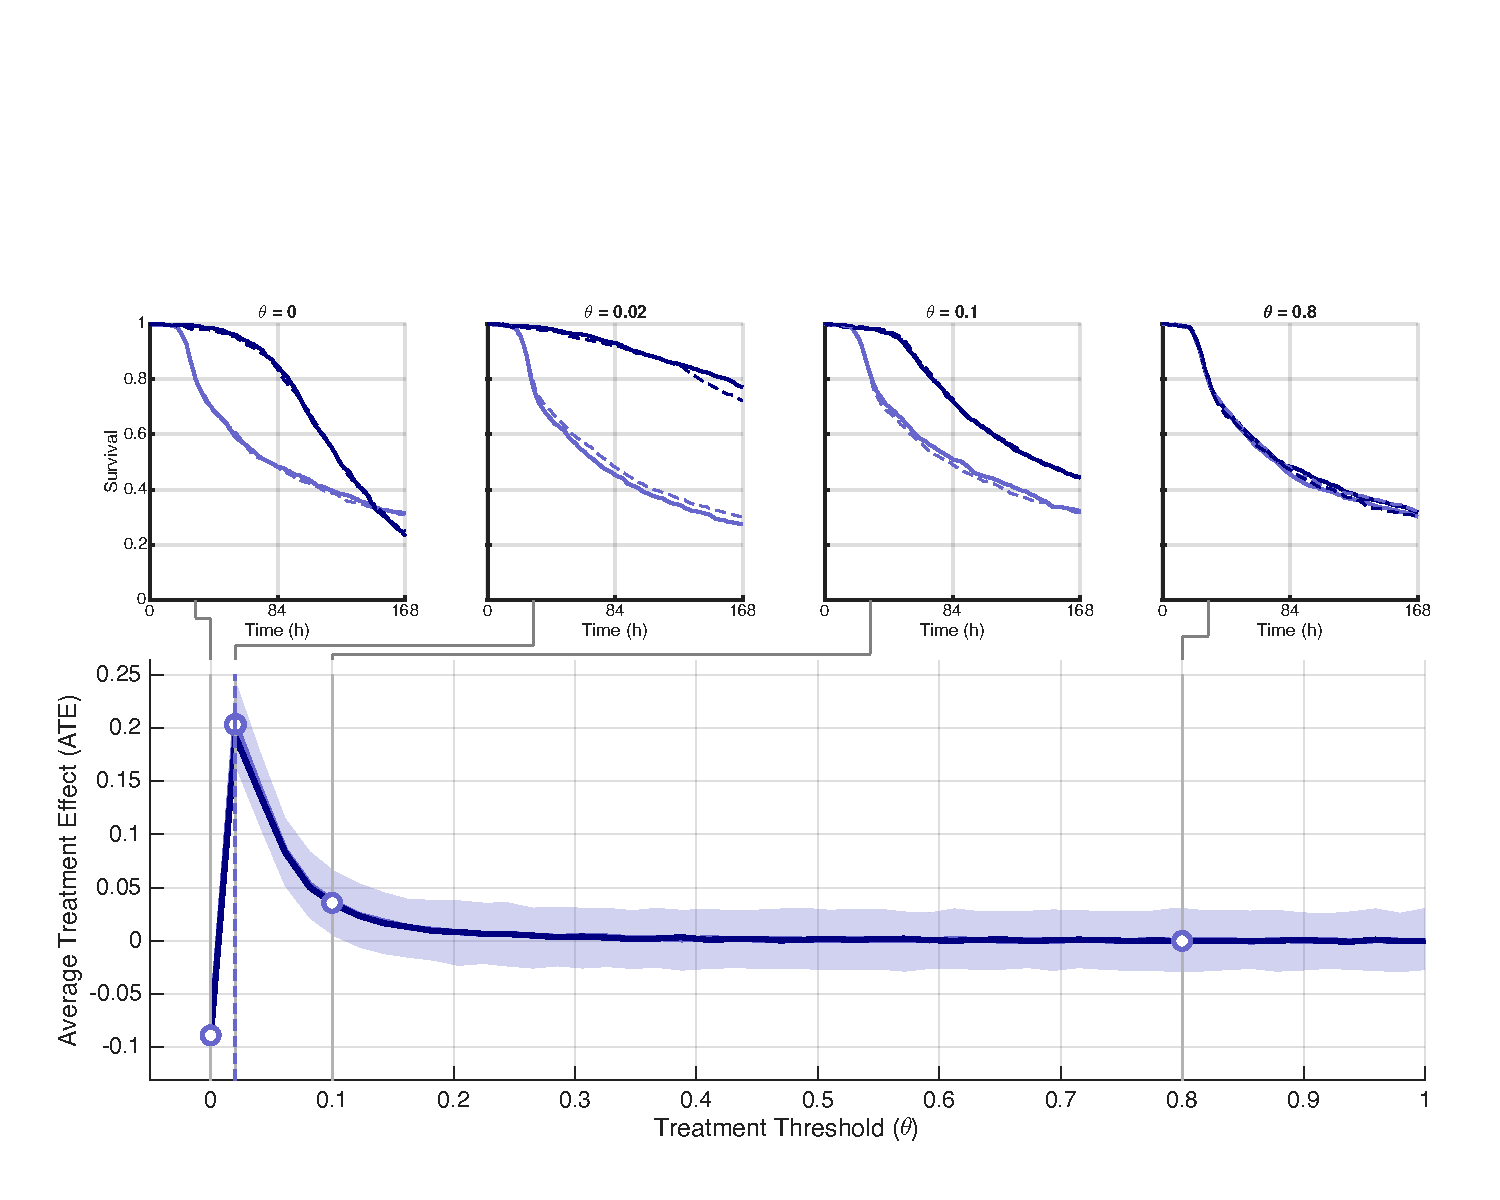
\includegraphics[width=\textwidth,height=0.40\textheight,keepaspectratio]{Fig_optimization_curves_with_survival.pdf}

\vspace{1.2em}

\noindent\textbf{(B) Policy contrast by simulated patient type}\par\vspace{0.2em}
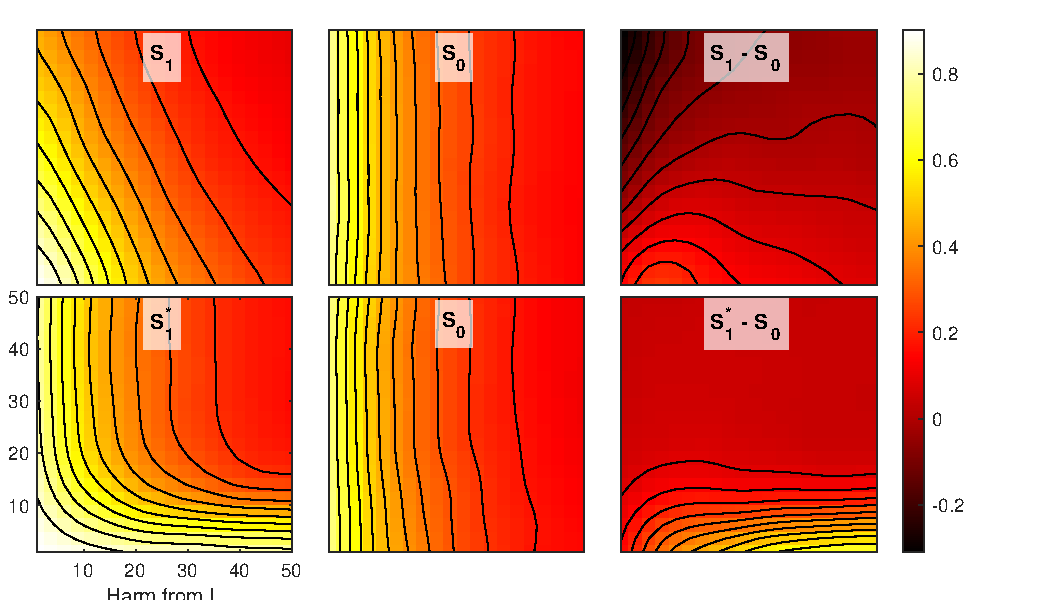
\includegraphics[width=\textwidth,height=0.40\textheight,keepaspectratio, trim=0pt 5pt 0pt 0pt, clip]{Fig_heatmap_figure.pdf}
\caption{\textbf{Exploring the space of closed-loop policies.} \textbf{(A)} Sweep over the family of
policies indexed by the target threshold $\theta$. Top: counterfactual survival curves under
different $\theta$. Bottom: policy contrast as a function of $\theta$, with the optimum of the
simulated process at $\theta = 0.02$ (contrast $+20.3\%$) and net toxicity under complete suppression
($\theta = 0$). The inverted-U shape reflects the benefit--toxicity trade-off specified in the
outcome model. \textbf{(B)} Policy contrast as a function of simulated patient type, indexed by
susceptibility to cumulative disease harm ($x$-axis) and cumulative drug harm ($y$-axis). Top row:
survival under treatment target $\theta = 0.1$ ($S_1$), under no treatment ($S_0$), and their
difference. Bottom row: survival under individualized optimal thresholds ($S_1^*$) and the
corresponding contrast $S_1^*-S_0$. The boundary separating benefit from harm is a direct consequence
of the two-parameter harm model and carries no information about where such a boundary would lie in
patients. All data are simulated.}
\label{fig:policy_space}
\end{figure}













































\subsection{Robustness Analyses}
\label{sec:robustness}

\paragraph{Robustness to unmeasured confounding.}
Across the \(5 \times 5\) (\(\delta_A\), \(\delta_Y\)) grid, with three seeds per cell at
\(N = 1500\) patients, the g-formula ATE retained the correct sign in every cell; no
sign flip was observed. The largest mean bias across cells was approximately
\(+10\) percentage points, at \((\delta_A = 0.5, \delta_Y = 0)\). The baseline (honest)
cell \((\delta_A = 0, \delta_Y = 0)\) showed a mean bias of about \(+4.6\) pp, which is
within the expected finite-sample seed variance at this \(N\) and illustrates the
intrinsic variability of the estimator rather than a systematic effect of \(U\).
Importantly, there is no monotonic pattern in which larger \(U\) effects produce larger
bias, suggesting that within the tested range the g-formula's estimate is primarily
noise-limited rather than bias-limited. The Ding--VanderWeele E-value for the honest ATE
was \(1.46\), meaning an unmeasured confounder would need a risk ratio of at least 1.46
with both treatment assignment and mortality to fully account for the observed effect.
Full results appear in \texttt{sensitivity/nuc\_injection/nuc\_results.mat}.

\paragraph{Robustness to EEG measurement error.}
Small amounts of measurement error on \(L_t\) had modest effect on the recovered ATE: at
\(\sigma = 0.025\) the bias remained within stochastic seed variability. Above
\(\sigma = 0.05\) the two-stage PKPD estimator fit-failed on a substantial fraction of
cohorts because the signal-to-noise ratio in \(L_t\) became too low for stable
identification of \(C_{50}\) and \(\gamma\). This sets a practical requirement that the
EEG-severity proxy used in the planned real-data analysis be measured with noise well
below this threshold.

\paragraph{Robustness to censoring mechanism.}
Under the baseline censoring regime used in the paper, the g-formula bias was
\(-0.6~\mathrm{pp}\) relative to the RCT truth. Under MCAR censoring at a low rate, bias
was approximately \(+8~\mathrm{pp}\); under strongly outcome-dependent censoring (5\% of
person-time censored in a manner correlated with both disease severity and treatment
intensity), bias grew to \(+17~\mathrm{pp}\). This sensitivity is expected: when
censoring is strongly informative and the observed data do not capture what drives
loss-to-follow-up, the g-formula's assumption of conditional independent censoring is
violated, and bias increases. For the planned real-data analysis, rigorous
characterization of the censoring mechanism (protocol deviations, withdrawal of care,
transfer out) will be essential.

\subsection{Methodological Benchmarking against IPTW, MSM, and Naive KM}
\label{sec:benchmark}
Table~\ref{tab:benchmark} reports the 168-hour ATE estimates from four methods on the same
simulated observational cohort (\(N = 2000\)), with 95\% bootstrap CIs.

\begin{table}[H]
\centering
\begin{tabular}{lrrr}
\toprule
Method                  & ATE at 168h & 95\% CI         & Bias vs truth \\
\midrule
RCT truth               & $+14.8\%$   & ---             & ---           \\
Naive Kaplan--Meier     & $-4.8\%$    & $[-11.4, -0.2]$ & $-19.6$~pp    \\
Stabilized IPTW         & $+16.6\%$   & $[+2.5, +27.4]$ & $+1.9$~pp     \\
MSM (baseline-weighted) & $+31.6\%$   & $[+17.2, +41.7]$& $+16.8$~pp    \\
\textbf{CICADAS g-formula} & $\mathbf{+14.5\%}$ & $[\mathbf{+7.4, +20.8}]$ & $\mathbf{-0.3~pp}$ \\
\bottomrule
\end{tabular}
\caption{Four-method comparison of 168-hour ATE recovery from the same simulated observational cohort. Bootstrap 95\% CIs: 200 replicates for naive KM/IPTW/MSM; 1000 replicates for the CICADAS g-formula. The CICADAS g-formula is the only estimator whose point estimate lies within one standard error of the RCT ground truth. All four estimators are computed on one shared cohort so that the comparison is like-for-like; the g-formula value here ($+14.5\%$) therefore differs slightly from the $+14.2\%$ reported in Section~\ref{sec:gformula-results}, which is computed on an independently simulated cohort. The 0.3-point difference is Monte Carlo variation between cohorts (Table~\ref{tab:multiseed}). All data are simulated.}
\label{tab:benchmark}
\end{table}

The CICADAS g-formula is the only estimator among the four whose point estimate is within
one standard-error of the RCT truth. IPTW is approximately correct but the propensity
model produced extreme weights (maximum 131; 99th percentile 2.74) reflecting
near-positivity violation for the continuous state-dependent dosing in this simulation.
This is empirical evidence for the conceptual argument made in Section~\ref{sec:positivity} that IPTW is
ill-suited to continuous-treatment dynamic policies over long horizons.

This comparison is methodological benchmarking, not evidence of clinical superiority. The g-formula
implementation here is correctly specified with respect to the process that generated the data, while
the IPTW and MSM implementations are standard off-the-shelf specifications; a comparison in which one
estimator knows the true functional form and its competitors do not is informative about
implementation, not about which method to prefer in real data. The IPTW result is nonetheless
instructive on its own terms: the propensity model produced extreme weights (maximum 131) reflecting
near-violation of positivity for continuous state-dependent dosing, and that difficulty is intrinsic
to the setting rather than to our implementation. In real data, where no method is correctly
specified, the ordering could differ. The MSM with
baseline-only stabilized weights is substantially biased, overestimating the ATE by
approximately 17 percentage points; a time-varying MSM that also reweights for time-
varying confounders would in principle do better, but would itself suffer from the same
near-positivity issue with extreme weights.
